\documentclass{article}
%\usepackage[utf8]{inputenc}
\usepackage[a4paper, total={7in, 8in}]{geometry}
\usepackage{spverbatim}
\usepackage{minted}
\usepackage{amssymb}
\usepackage{bm}
\usepackage{graphicx}

\usepackage{amsmath}
\usepackage{halloweenmath}


\title{EECE 7205-Assignment1}
\author{Sreejith Sreekumar: 001277209}
\date{\today}
\begin{document}

\maketitle
\section{Coding}
\subsection{Insertion Sort}

\begin{minted}{C++}
#include <iostream>
#include <time.h>


int *get_input(int limit){
  
   /**
    * Generating input - Worst case happens when the array is sorted in
    * reverse order. Sending numbers from 1000 to limit 
    * decrementing by 1 for every element.
    */
    
  int* input = new int[limit];

  int j = 0;
  for(int i=1000; i>1000-limit; i--){
    input[j] = i;
    j+=1;
  }
  return input;
}


int *insertion_sort(int input[], int limit){
  
   /**
    * Insertion sort algorithm
    */
    
  int i, j, temp;
  for (i=0; i< limit; i++){
    for (j=i ;j>=0; j--){
      if(input[j] < input[j-1]){
	temp = input[j];
	input[j] = input[j-1];
	input[j-1] = temp;
      }
    }
  }
  return input;
}


int main(){

  int limit, i;
  std :: cout <<"Enter limit: ";
  std :: cin>> limit;

  int* input = get_input(limit);
  
  /*
   * Setting clocks before and after the sorting
   */
  clock_t start = clock();
  int* sorted_array = insertion_sort(input, limit);
  clock_t end = clock();

  double cpu_time_used = ((double) (end - start)) / CLOCKS_PER_SEC;

  std::cout<< "Insertion Sort took %f seconds to finish \n" << cpu_time_used;
  
}

\end{minted}

\subsection{Merge Sort}
\begin{minted}{C++}
#include <iostream>
#include <time.h>

int *get_input(int limit){

   /**
    * Generating input - Worst case - Sending numbers from 1000 to limit 
    * decrementing by 1 for every element.
    */
    
  int* input = new int[limit];

  int j = 0;
  for(int i=1000; i>1000-limit; i--){
    input[j] = i;
    j+=1;
  }
  return input;
}


void copy_merged_array_into_original(int original[], int merged[], int length, int left_low) {

    for (int i=0; i< length; ++i)
        original[left_low++] = merged[i];
        
}


void merge(int input[], int left_low, int left_high, int right_low, int right_high) {

    int length = right_high-left_low+1;
    int merged_array[length];
    int left = left_low;
    int right = right_low;

    auto left_array_exhausted = [&left, &left_high]() { return left > left_high;};
    auto right_array_exhausted = [&right, &right_high]() { return right > right_high;};

    for (int i = 0; i < length; ++i) {
        if (left_array_exhausted())
            merged_array[i] = input[right++];
        else if (right_array_exhausted())
            merged_array[i] = input[left++];
        else if (input[left] <= input[right])
            merged_array[i] = input[left++];
        else
            merged_array[i] = input[right++];
    }
    copy_merged_array_into_original(input,  merged_array, length, left_low);

}


void merge_sort(int numbers[], int low, int high) {

    if (low >= high)
        return;

    else {
    
        /*
         * Recursive sorting and merging parts
         */
         
        int mid = (low + high)/2;
        merge_sort(numbers, low, mid);
        merge_sort(numbers, mid+1, high);
        merge(numbers, low, mid, mid+1, high);
    }

}


int main(){


    int limit;
    
    std :: cout << "Enter limit: ";
    std :: cin >> limit;

    int* input = get_input(limit);
    std :: cout << "Sorting using mergesort: ";
    
  /*
   * Setting clocks before and after the sorting
   */    
    clock_t start = clock();
    merge_sort(input, 0, limit-1);
    clock_t end = clock();

    double cpu_time_used = ((double) (end - start)) / CLOCKS_PER_SEC;
    cout << "Merge Sort took %f seconds to finish \n" << cpu_time_used;

}

\end{minted}


\pagebreak

\subsection{Worst Case Running Times}

Experimenting using the above code fragments which sorts using insertion and mergesort for different values of 'n' at their worst cases, we have:
at \textbf{n=43}, mergesort starts to beat insertion sort (ref. Figure 1).

\begin{figure}
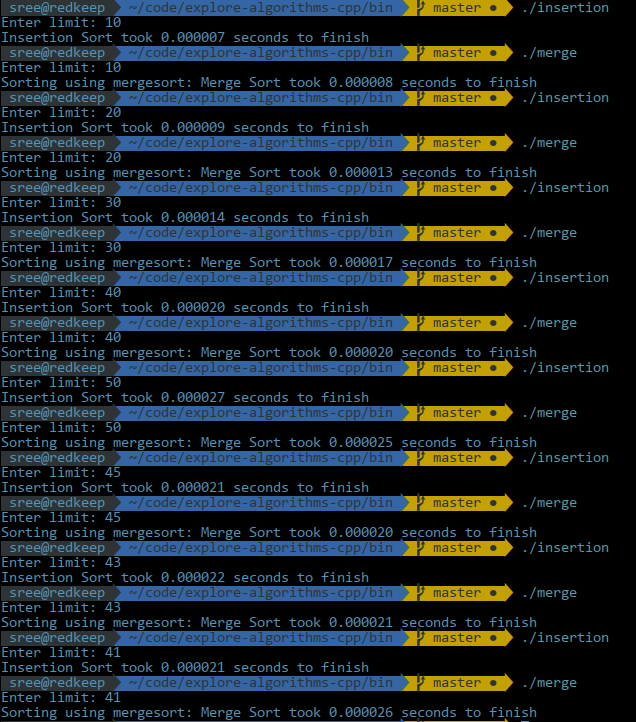
\includegraphics[width=10cm]{expt.png}
\caption{Sorting Algorithms - Running time experiments}  
\end{figure}

\section{Arrangement of Elements during Sorting}
\subsection{Insertion Sort}
\begin{minted}{Python}
Input: {10, 5, 7, 9, 8, 3}
Iteration 1: {5, 10, 7, 9, 8, 3}
Iteration 2: {5, 7, 10, 9, 8, 3}
Iteration 3: {5, 7, 9, 10, 8, 3}
Iteration 4: {5, 7, 9, 8, 10, 3}
             {5, 7, 8, 9, 10, 3}
Iteration 5: {5, 7, 8, 9, 3, 10}
             {5, 7, 8, 3, 9, 10}
             {5, 7, 3, 8, 9, 10}
             {5, 3, 7, 8, 9, 10}
             {3, 5, 7, 8, 9, 10}
             
  Final    : {3, 5, 7, 8, 9, 10}             
\end{minted}

\subsection{Quicksort}
Input: {10, 5, 7, 9, 8, 3} \\
\begin{minted}{Python}
  Pivot: 10
  
  Iteration 1: {->10, 5, 7, 9, 8, 3}
              Exchange Pivot
               {3, 5, 7, 9, 8, 10}
  Iteration 2: {->3, 5, 7, 9, 8, 10}
  Iteration 3: {3, ->5, 7, 9, 8, 10}
  Iteration 4: {3, ->5, 7, 9, 8, 10}
  Iteration 5: {3, 5, ->7, 9, 8, 10}
  Iteration 6: {3, 5, 7, ->9, 8, 10}
              Exchange Pivot
              {3, 5, 7, 8, 9, 10}
              
  Final      : {3, 5, 7, 8, 9, 10}
\end{minted}

\section{True or False}

\begin{itemize}
\item n + 3 $\in$ $\Omega$(n) - True

\item n + 3 $\in$ $\mathcal{O}(n^{2})$ - True

\item n + 3 $\in$ $\Theta(n^{2})$ - False

\item $2^{n+1}$ $\in$ $\mathcal{O}$(n + 1) - False

\item $2^{n+1}$ $\in$ $\Theta(2^{n})$ - True

\end{itemize}

\section{Master Method}

\begin{itemize}
\item T(n) = 8T($\frac{n}{2}$) + n \\ \\
  Here a = 8, b = 2 and f(n) = n \\
  Considering Case I of the Master Method, i.e $\mathcal{O}(n^{\log_b {a} - \varepsilon})$ and substituting for a and b, we have: \\

  f(n) = n = $\mathcal{O}(n^{\log_2 {8} - \varepsilon})$ =  $\mathcal{O}(n^{3 - \varepsilon})$ \\

  For $\varepsilon$ = 1, we have f(n) = $\mathcal{O}(n^{2})$, which satisfies Case I \\

  $\therefore$ T(n) = $\Theta(n^{\log_b {a}})$ = $\Theta(n^{3})$




\item T(n) = 8T($\frac{n}{2}$) + $n^{2}$ \\ \\
  Here a = 8, b = 2 and f(n) = $n^{2}$ \\
  Considering Case I of the Master Method, i.e $\mathcal{O}(n^{\log_b {a} - \varepsilon})$ and substituting for a and b, we have: \\

  f(n) = $n^{2}$ = $\mathcal{O}(n^{\log_2 {8} - \varepsilon})$ =  $\mathcal{O}(n^{3 - \varepsilon})$, which satisfies Case I \\

  $\therefore$ T(n) = $\Theta(n^{\log_b {a}})$ = $\Theta(n^{3})$




\item T(n) = 8T($\frac{n}{2}$) + $n^{3}$ \\ \\
  Here a = 8, b = 2 and f(n) = $n^{3}$ \\
  Considering Case II of the Master Method, i.e $\Theta(n^{\log_b {a}})$ and substituting for a and b, we have: \\

  f(n) = $n^{3}$ = $\Theta(n^{\log_2 {8}})$ =  $\Theta(n^{3})$, which satisfies Case II \\

  $\therefore$ T(n) = $\Theta(n^{\log_b {a}}.log n)$ = $\Theta(n^{3} log n)$
  


  
\item T(n) = 8T($\frac{n}{2}$) + $n^{4}$ \\ \\

  Here a = 8, b = 2 and f(n) = $n^{4}$ \\
  Considering Case III of the Master Method, i,e $\Omega(n^{\log_b {a} + \varepsilon})$ and substituting for a and b, we have: \\

  \begin{equation}
    f(n) = n^{4} = \Omega(n^{\log_2 {8} + \varepsilon}) =  \Omega(n^{3 + \varepsilon})   \\
  \end{equation}

  and,
  
  \begin{equation}
    8.f(\frac{n}{2}) \leq (1 - \varepsilon^{\prime}).n^{4}
   \end{equation}

  \begin{equation}
  \implies 8.\frac{n^{4}}{16} \leq (1 - \varepsilon^{\prime}).n^{4}
  \end{equation}

  \begin{equation}
  \implies \frac{n^{4}}{2} \leq (1 - \varepsilon^{\prime}).n^{4}    
  \end{equation}
  
  (1) is true for many $\varepsilon^{\prime}s$ $>$ 1
  and (4) is true for 0 $<$ $\varepsilon^{\prime}$ $<$ 0.5
  
  From (1) and (4) Master Method Case III is satisfied.

  $\therefore$ T(n) = $\Theta$(f(n)) = $\Theta(n^{4})$

\end{itemize}

\\

\\

(Happy Halloween \mathwitch)


\section{Recursion Tree}
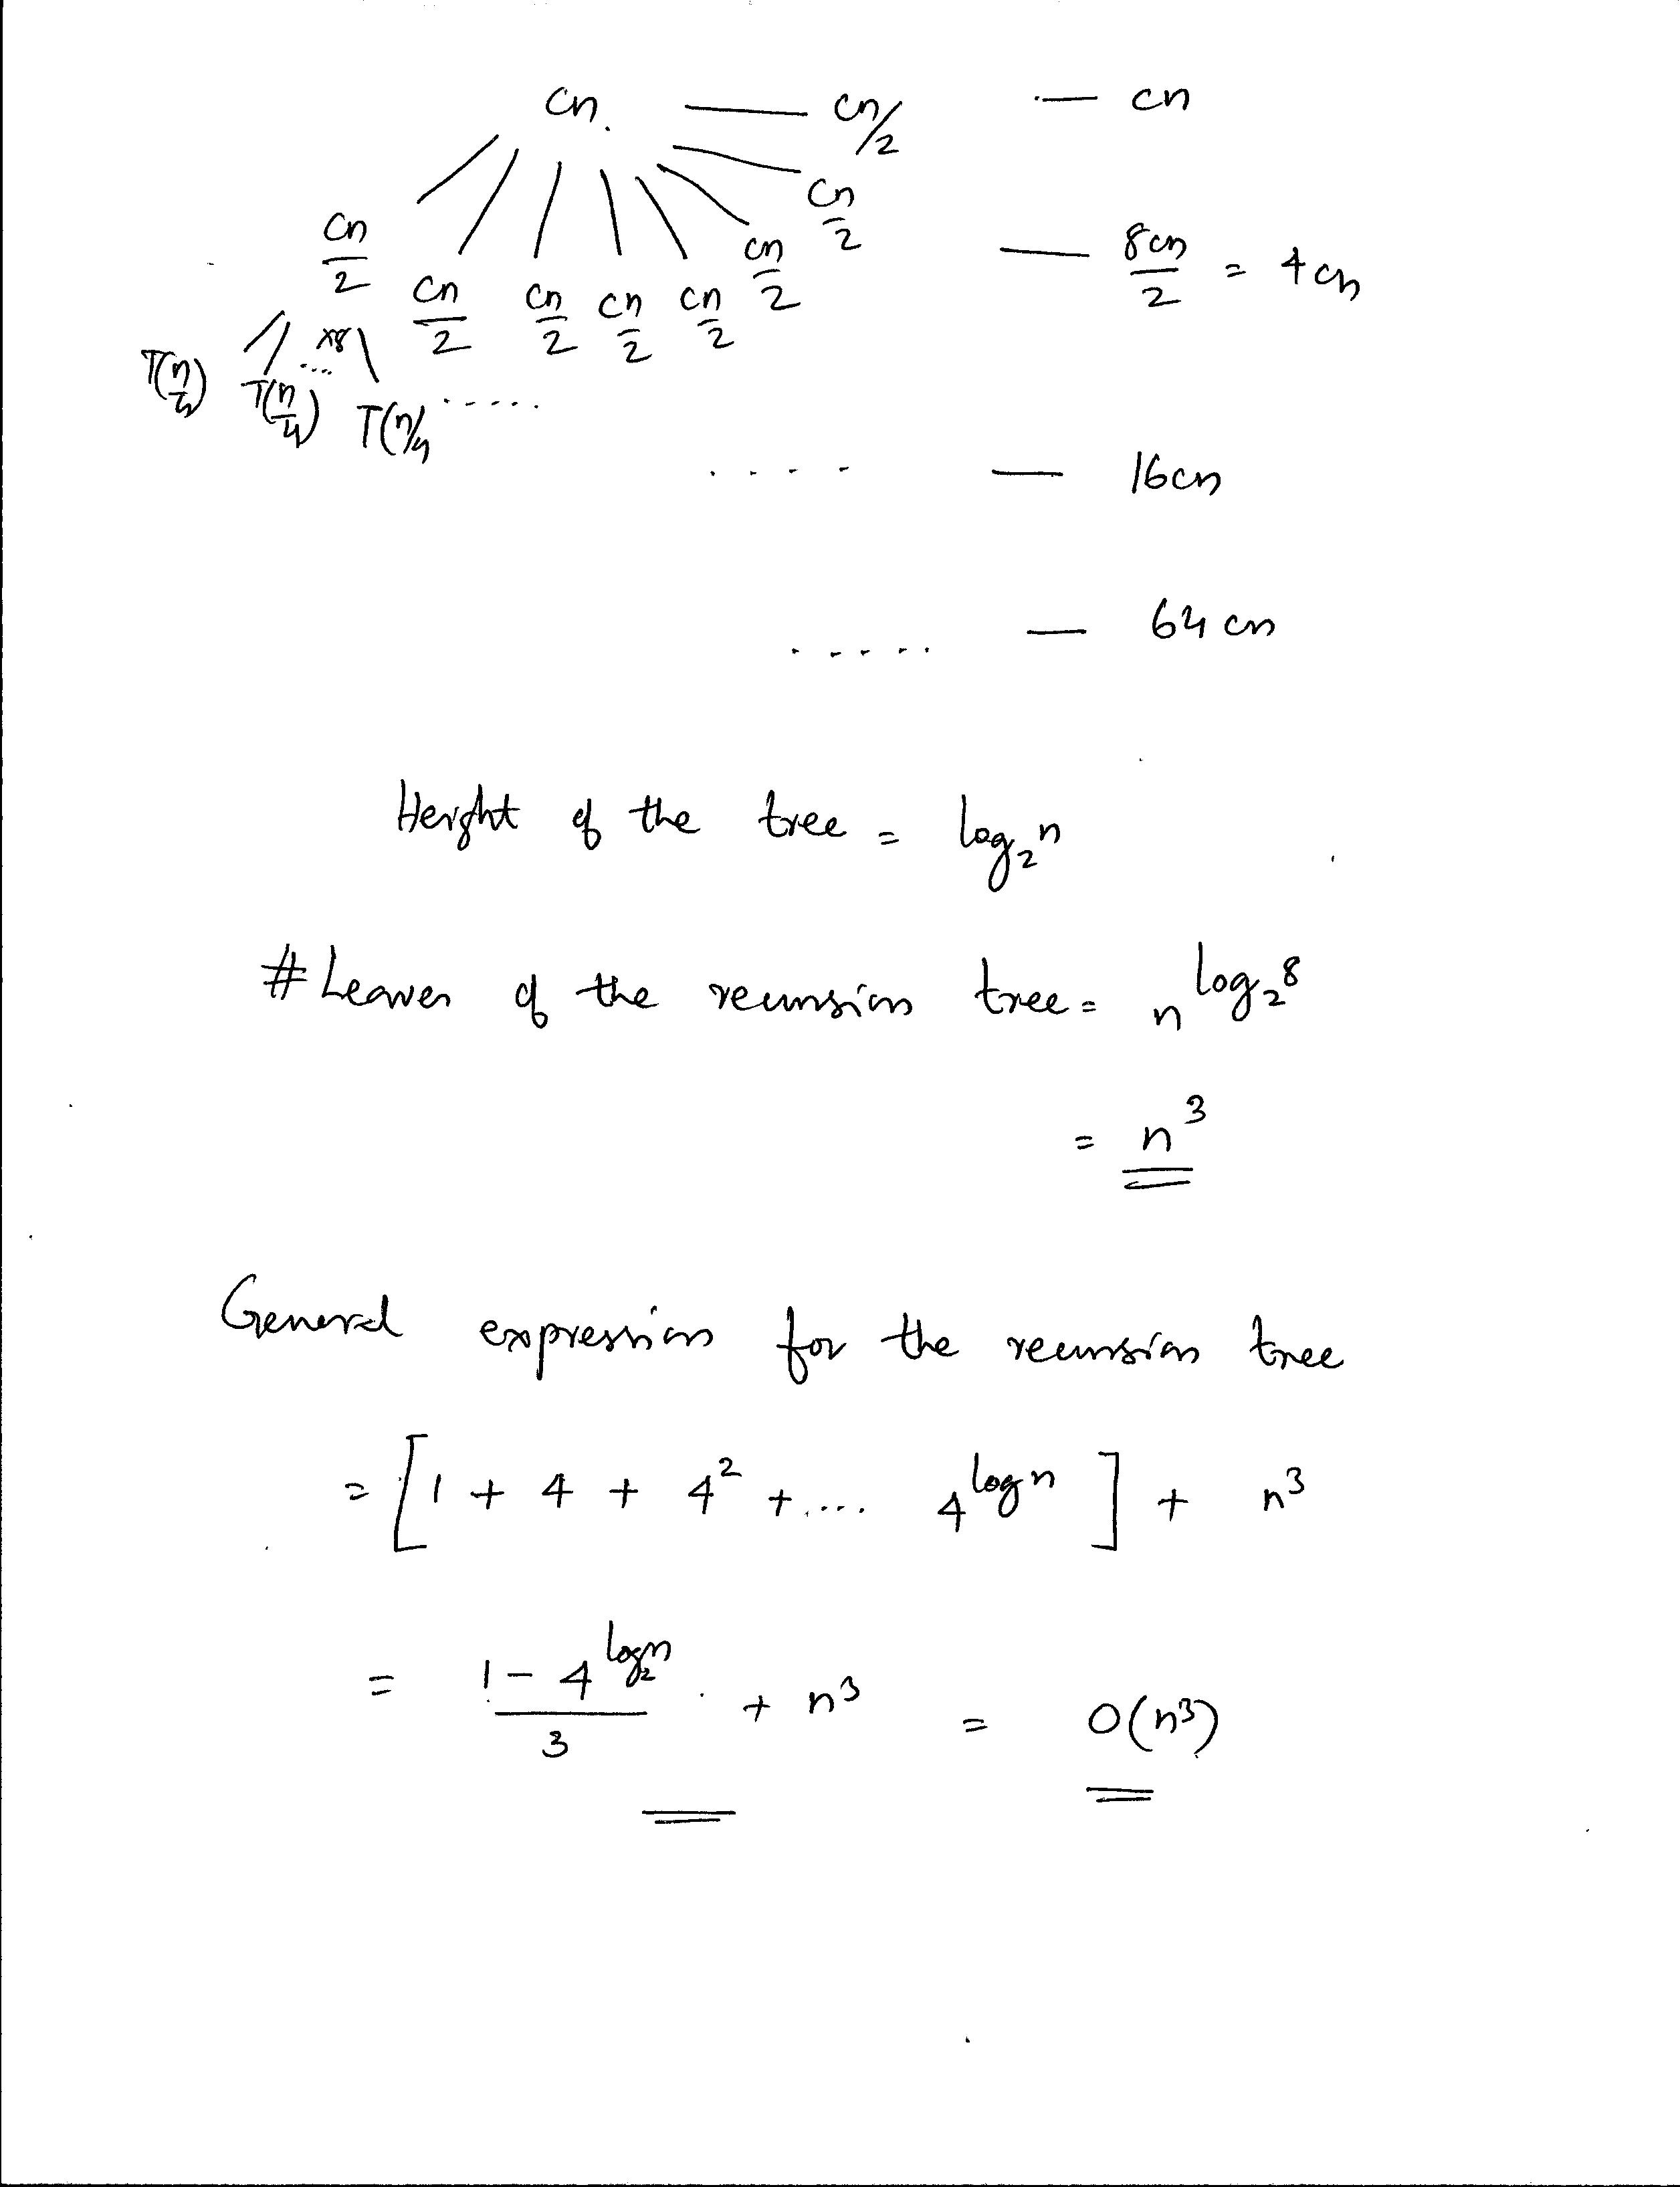
\includegraphics[width=20cm]{page1.jpg}
\linebreak
\pagebreak

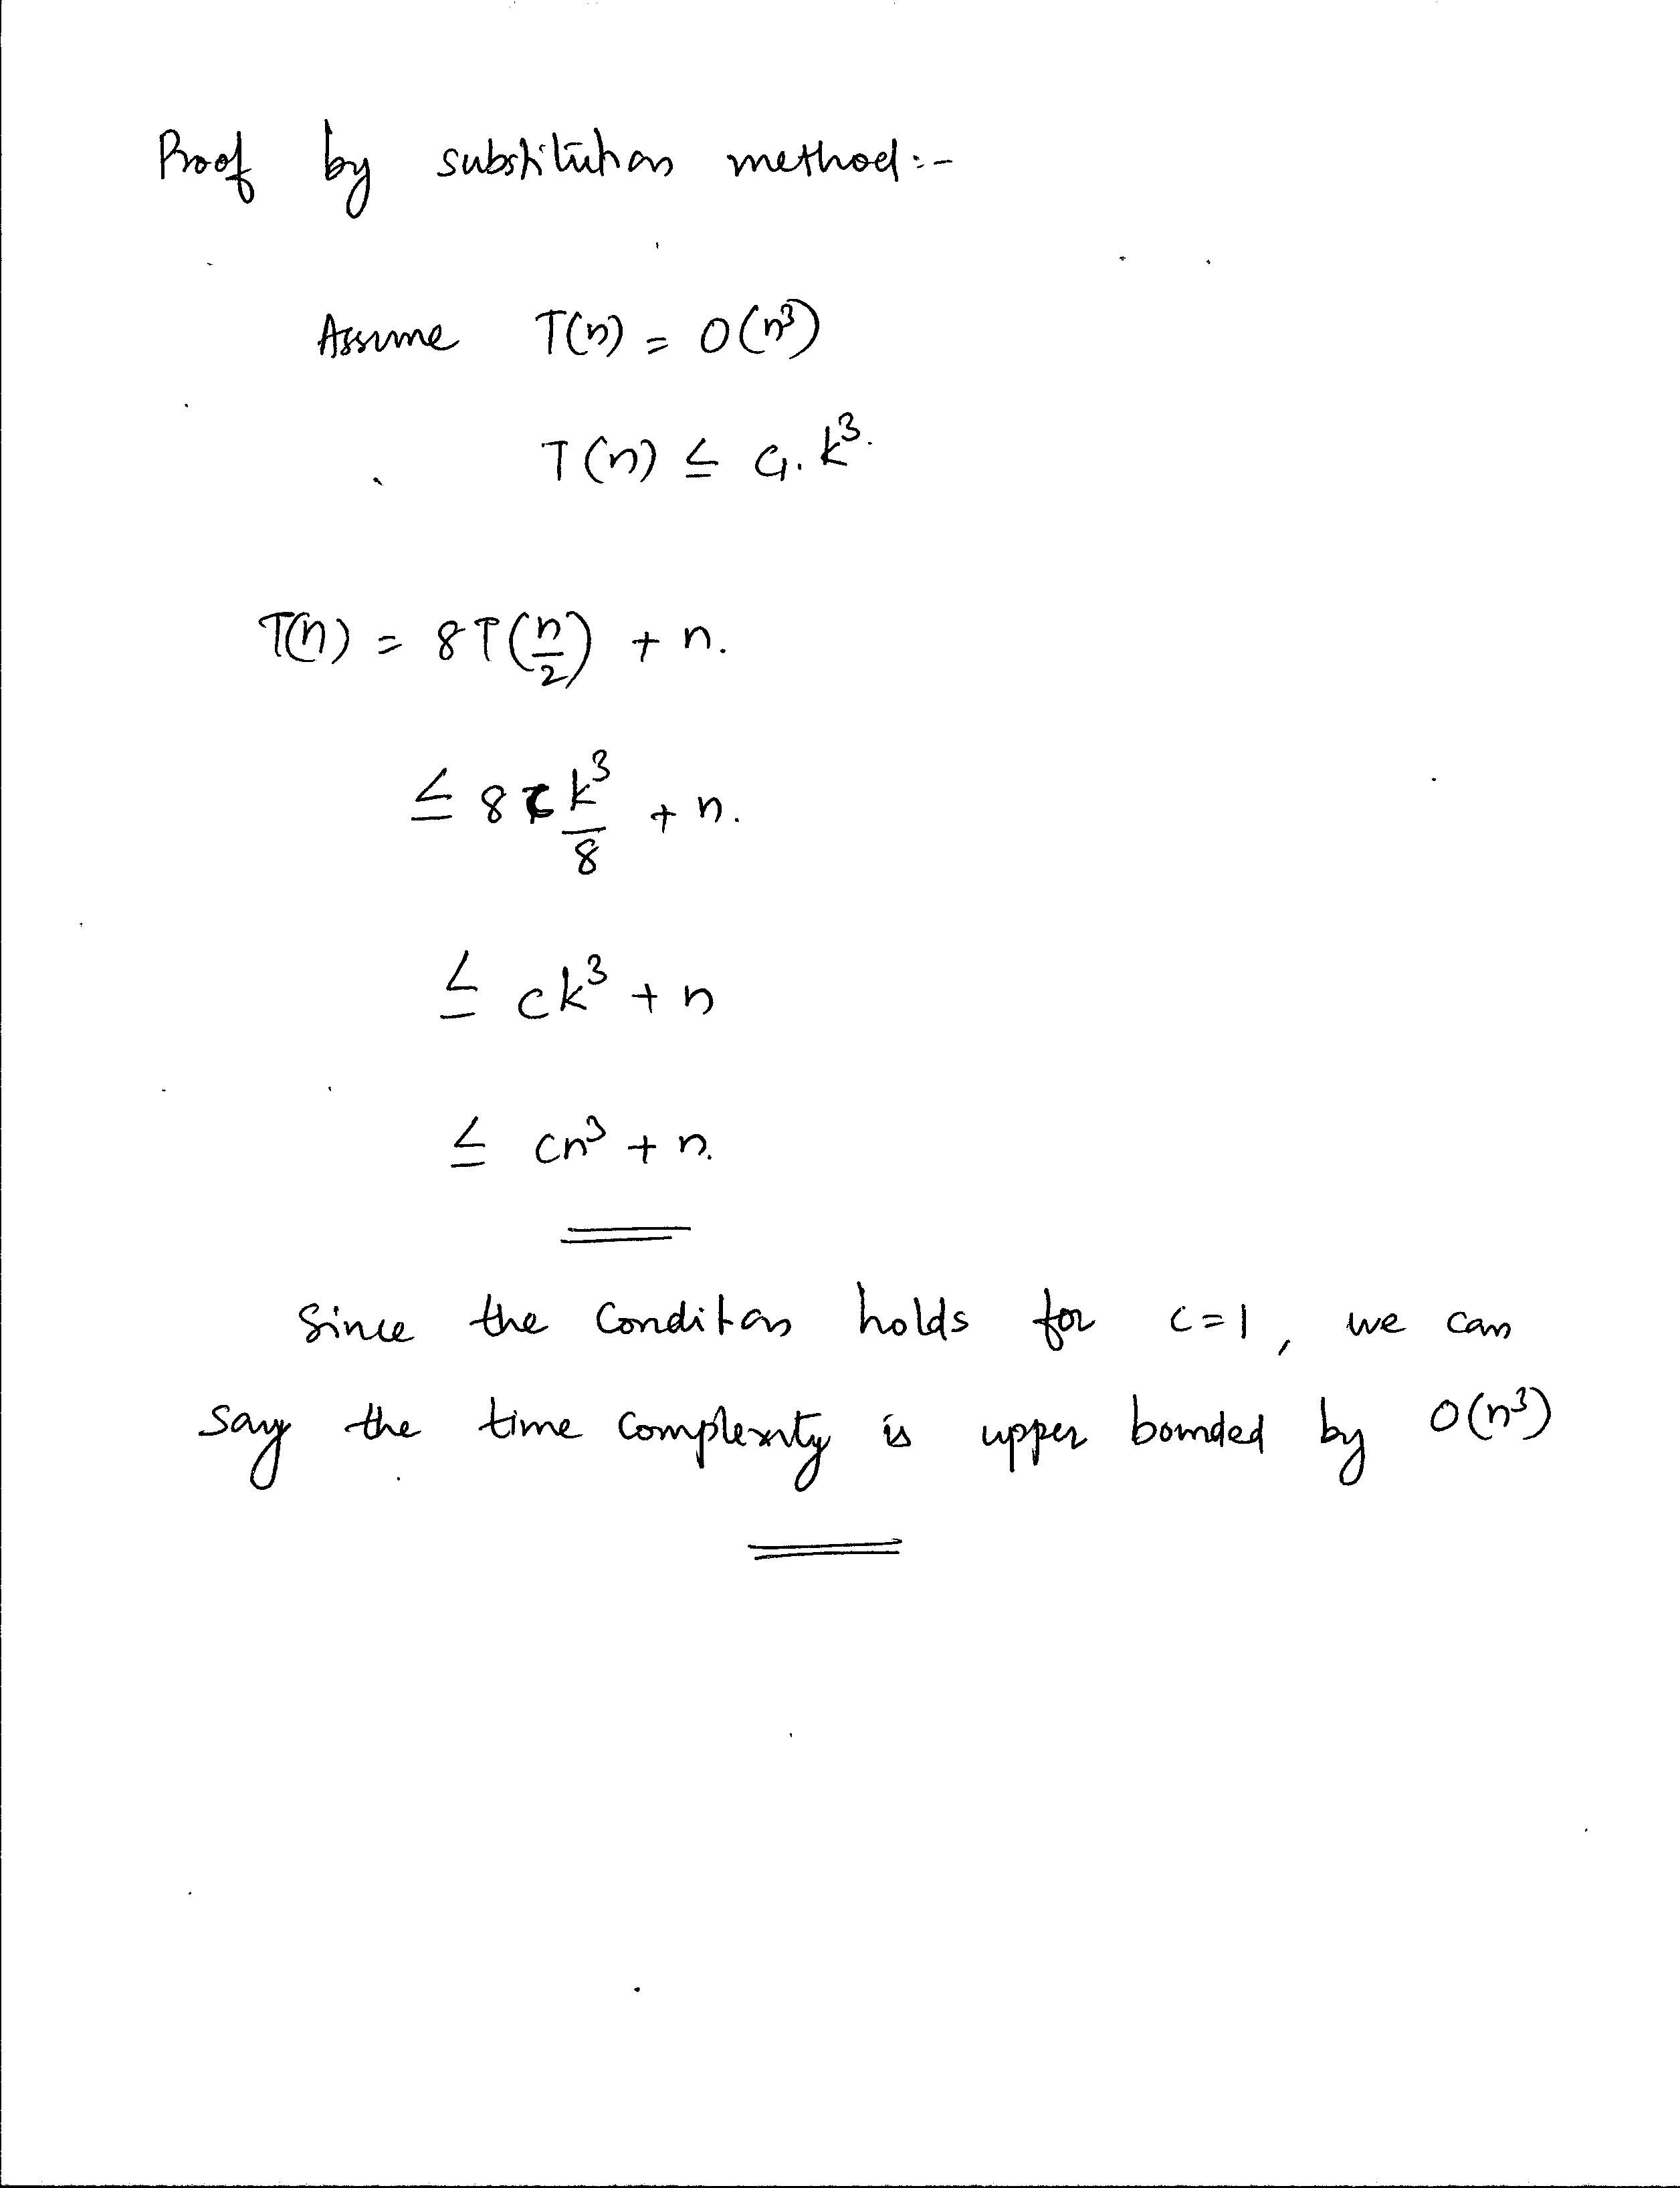
\includegraphics[width=20cm]{page2.jpg}




\end{document}











